\documentclass[11pt,spanish]{article} % Tipo y tamaño de letra del documento.


\usepackage[utf8]{inputenc}
\usepackage{subfiles}
\usepackage{biblatex}
\addbibresource{references.bib}
\usepackage{multicol}
\usepackage{amsfonts}
\usepackage{blindtext}
\usepackage{mathrsfs}
\usepackage{amsmath}
\usepackage{siunitx}
\usepackage{centernot}
\usepackage[shortlabels]{enumitem}
\usepackage{subfig}
\usepackage{datetime}
\usepackage{listingsutf8}
\usepackage[spanish]{babel}
\usepackage{tikz}
\usepackage{hyperref}
\usepackage[vlined,ruled,linesnumbered]{algorithm2e}
\usepackage{listings}
\usepackage{float}
\usepackage{url}
\usepackage{csquotes}
\usepackage{fourier} %font
\usepackage[top=2cm, bottom=2cm, left=2.5cm, right=2.5cm]{geometry}
\usepackage{pgfplots}
\usepackage{fancyhdr}
\usepackage{mdframed}
\usepackage{tikzducks}
\usepackage[nameinlink]{cleveref}
\usepackage{epigraph} 

\pgfplotsset{compat=1.18}

\usetikzlibrary{shapes.arrows, shapes.geometric, arrows.meta,angles,quotes,positioning,arrows,fit,quotes,calc}
\tikzset{>=latex} 

\setlength\algomargin{1em} 
\SetFuncSty{sc} 
\SetCommentSty{em} 


\Crefname{figure}{Fig.}{Figs.}
\newcommand\crefrangeconjunction{--}
\Crefname{table}{Tabla}{Tablas}
\Crefname{subsubsection}{Subsubsec.}{Subsubsections}
\Crefname{subsection}{Subsec.}{Subsections}
\Crefname{section}{Sec.}{Sections}
\Crefname{equation}{eq.}{eqs.}
\crefname{thm}{Theorem}{theorems}
\Crefname{thm}{Theorem}{Theorems} 

\definecolor{algoco}{rgb}{0,0.0,1}

\hypersetup{
  colorlinks=true,
  linkcolor=algoco,
  citecolor=blue,
  urlcolor=blue,
}

\lstset{
extendedchars=true
inputencoding=utf8/latin1,
basicstyle=\footnotesize\sffamily\color{black},
commentstyle=\slshape \color{gray},
numbers=left,
numbersep=10pt,
numberstyle=\tiny\color{red!80!black},
keywordstyle=\color{red!80!magenta},
showspaces=false,
showstringspaces=false,
stringstyle=\color{cyan!80!black},
tabsize=2,
literate={á}{{\'a}}1 {é}{{\'e}}1 {í}{{\'i}}1 {ó}{{\'o}}1 {ú}{{\'u}}1,
frame = single, 
numbers = none,
float, floatplacement = ht, captionpos = b,
xleftmargin = 2em, xrightmargin = 2em, 
}

\newcommand{\ub}[1]{\underbrace{#1}}
\newcommand\tcm{\textcolor{blue}}
\newcommand\tca{\textcolor{algoco}}

\setlength\epigraphwidth{.7\textwidth} 

\newcommand{\tnum}{2 y 3} % reemplace 2 por el número de la tarea
\newcommand{\sem}{2025-1} % reemplace 2024-2 por el semestre correspondiente
\newcommand{\campus}{San Joaquin \\ Santiago} % reemplace Casa Central por el campus correspondiente
\newcommand{\rolusm}{202173639-5} % reemplace 2025073100-1 por su rol
\newcommand{\namestudent}{Renato Ramírez} % reemplace Al Goritmo Pérez por su nombre

\headheight=14pt
\linespread{1.3}
\author{\namestudent}
\pagestyle{fancy}
\fancyhf{}%
\fancyfoot[R]{ \namestudent \\ \rolusm}
\fancyfoot[L]{Campus \campus} 
\fancyfoot[C]{\thepage}
\rhead{\sem}
\lhead{INF-221}
\renewcommand{\headrulewidth}{0.4pt}
\renewcommand{\footrulewidth}{0.4pt}
\newbool{programs}
\boolfalse{programs}
\chead{REPORTE TAREA \tnum~}



\title{
  \huge
  \textbf{REPORTE TAREA \tnum~ \\ ALGORITMOS Y COMPLEJIDAD} \\[1ex]
  \emph{\textquote{Más allá de la notación asintótica: Análisis experimental de algoritmos de ordenamiento y multiplicación de matrices.}} 
  }

  
\date{
  \small
  \today\\
  \currenttime
}




\begin{document}
\maketitle
\thispagestyle{fancy} 
\vspace{-1.0\baselineskip}




\begin{abstract}
  \textit{ 
    En el mundo informático y en el cotidiano, el papel de los algoritmos es primordial,
pues permiten resolver problemas complejos de manera eficiente y automática. Un
algoritmo puede entenderse como un conjunto de instrucciones que permiten,
mediante datos de entrada, conseguir datos de salida, es decir, es la función que
permite llegar de un conjunto de datos a una solución.
El desarrollo y análisis de algoritmos no solo se enfoca en encontrar soluciones
correctas, sino también en mejorar su rendimiento. Factores como la velocidad de
ejecución, el uso de recursos y la escalabilidad son determinantes para la eficiencia de
un algoritmo. En un mundo cada vez más conectado, donde el volumen de datos y la
complejidad de las tareas crecen de manera exponencial, diseñar algoritmos
eficientes se ha convertido en una prioridad clave.
Este informe tiene como objetivo explorar dos tipos de algoritmos, el de Ordenamiento,
es decir, ordenar los datos numéricos dentro de un vector, y de Multiplicación de
matrices. Para cada tipo se hará uso de varios algoritmos con el mismo fin y se
compararan en distintos escenarios para evaluar su rendimiento y su complejidad.\cite{elsevier_abstract_2024}.

  }
     
\end{abstract}

\setcounter{tocdepth}{1}
\tableofcontents


\newpage
\section{Introducción}
El an\'alisis y dise\~no de algoritmos es una de las bases fundamentales en la formaci\'on de estudiantes en Ciencias de la Computaci\'on. Comprender c\'omo se comportan distintos algoritmos en la pr\'actica permite tomar mejores decisiones sobre cu\'ando y por qu\'e utilizar uno u otro. En este trabajo se busca evaluar el rendimiento de dos enfoques para resolver un problema cl\'asico: encontrar las diferencias entre dos secuencias.

El problema de encontrar las diferencias entre dos secuencias consiste en identificar las partes no coincidentes entre ambas, resaltando al mismo tiempo las similitudes. Para lograr esto, se suele buscar la subsecuencia común más larga (LCS), y luego, con base en esa referencia, segmentar las porciones que no coinciden. Esta tarea es útil en áreas como el control de versiones, la comparación de textos o secuencias biológicas, donde es importante entender cómo y dónde dos cadenas difieren.

Para ello, se comparan dos estrategias distintas: una implementaci\'on por fuerza bruta, que explora todas las posibles subsecuencias para encontrar la subsecuencia com\'un m\'as larga, y otra basada en programaci\'on din\'amica, que utiliza una soluci\'on eficiente construyendo una tabla de subproblemas. Ambos enfoques fueron implementados y puestos a prueba en diferentes casos.

El objetivo principal de este informe es analizar cu\'ales son las diferencias pr\'acticas entre ambos algoritmos, en t\'erminos de tiempo de ejecuci\'on y uso de memoria. Para ello, se desarroll\'o una serie de experimentos que permiten observar hasta qu\'e punto es viable usar fuerza bruta y cu\'al es el comportamiento real de la programaci\'on din\'amica en escenarios m\'as exigentes.

Este tipo de comparaci\'on no busca ser un aporte novedoso a la literatura cient\'ifica, sino una herramienta de aprendizaje. A trav\'es de este informe, se espera poner en pr\'actica los conocimientos adquiridos en el curso, como el an\'alisis de eficiencia, la complejidad algor\'itmica y el dise\~no de experimentos.



\newpage
\section{Implementaciones}
Todo el código utilizado para la elaboración de este informe, ademas de los algoritmos utilizados, mediciones, etc. Se encuentran en el siguiente repositorio de Github:

\begin{mdframed}
    \begin{center}
        {\Large \url{https://github.com/xReNatS/INF221-2025-1-TAREA-1}}
    \end{center}
\end{mdframed}




\newpage
\section{Experimentos}
En esta sección se describen la infraestructura utilizada y los casos de prueba que sustentan el análisis experimental. Nuestro objetivo es garantizar la reproducibilidad y entender las condiciones bajo las cuales se obtuvieron los resultados.

Para la ejecución de las pruebas se utilizó con computador de escritorio con las siguientes características: procesador Intel(R) Core(TM) i5-7400 CPU @ 3.00GHz   3.00 GHz, 16 GB de memoria DDR4, almacenamiento SSD NVMe y sistema operativo Windows 11 pro. Todas las implementaciones se compilaron con g++ 14.2.0 usando la optimización \texttt{-O2}. Para la generación de gráficos se utilizó Python 3.10 con numpy, pandas, matplotlib y la libreria seaborn para el diseño.




\subsection{Dataset (casos de prueba)}
Los casos de prueba que fueron utilizados cubren las cuatro dimensiones especificadas para cada problema: tamaño de entrada (\(n\)), tipo de estructura o disposición (\(t\)), dominio de valores (\(d\)) y réplica de muestra (\(m\)). A continuación se comentan ambos grupos de casos.

\subsubsection{Multiplicación de matrices}
\begin{itemize}
  \item \textbf{Tamaños (\(n\))}: \(\{2^4,\,2^6,\,2^8,\,2^{10}\}\).  
    Estos valores permiten medir cómo escalan el tiempo (\(O(n^3)\) vs. \(O(n^{\log_2 7})\)) y el uso de memoria con el crecimiento de la dimensión.
  \item \textbf{Tipos (\(t\))}: \{\emph{densa}, \emph{diagonal}, \emph{dispersa}\}.  
    Cada estructura permite evaluar el rendimiento en escenarios de cómputo completo, optimización para ceros en diagonal y aprovechamiento de la dispersión de datos.
    \begin{itemize}
      \item \emph{Densa}: coeficientes aleatorios no nulos, representa el peor caso de cómputo completo.  
      \item \emph{Diagonal}: matrices con solo la diagonal principal distinta de cero, evalúa cómo afectan las optimizaciones en cero.  
      \item \emph{Dispersa}: pocos elementos no nulos distribuidos aleatoriamente, comprueba si el overhead de recursión amortiza el cálculo en estructuras crestas.  
    \end{itemize}
  \item \textbf{Dominio (\(d\))}: \(\{D0,\,D10\}\), con  
    \(D0=\{0,1\}\) y \(D10=\{0,\dots,9\}\).  
    Esta variación confirma que los algoritmos mantienen su comportamiento sin depender de la amplitud del dominio.
  \item \textbf{Muestras (\(m\))}: \(\{a,b,c\}\).  
    Tres réplicas para cada combinación permiten calcular varianza y construir intervalos de confianza de tiempo y memoria.
  \item \textbf{Generación}: los archivos fueron producidos con \texttt{matrix\_generator.py} 
  
  (en \texttt{code/matrix\_multiplication/scripts/}), de manera que se pueda reproducir lo experimentado.
\end{itemize}

\subsubsection{Ordenamiento}
\begin{itemize}
  \item \textbf{Tamaños (\(n\))}: \(\{10^1,\,10^3,\,10^5,\,10^7\}\).  
    Con ellos se mide el desempeño desde vectores muy pequeños hasta grandes, comparando \(O(n\log n)\) frente a \(O(n^2)\).
  \item \textbf{Tipos (\(t\))}: \{\emph{aleatorio}, \emph{ascendente}, \emph{descendente}\}.  
    Cada disposición corresponde a caso promedio, mejor y peor, permitiendo analizar la robustez de los algoritmos.
  \item \textbf{Dominio (\(d\))}: \(\{D1,\,D7\}\), donde  
    \(D1=\{0,1\}\) y \(D7=\{0,\dots,10^7\}\).  
    Esto asegura que las comparaciones no se vean afectadas por la dispersión de valores.
  \item \textbf{Muestras (\(m\))}: \(\{a,b,c\}\).  
    Tres instancias aleatorias para cada caso permiten estimar la variabilidad estadística de tiempos y consumos.
  \item \textbf{Generación}: los vectores fueron creados con \texttt{array\_generator.py} (en \texttt{code/sorting/scripts/}), asegurando que las pruebas coincidan con el repositorio oficial.
\end{itemize}


\subsection{Resultados}
En esta sección se presentan los resultados experimentales obtenidos al medir el tiempo de ejecución y el uso de memoria de las implementaciones de los algoritmos de fuerza bruta y programación dinámica para la detección de diferencias entre dos secuencias. Los datos fueron generados utilizando scripts en Python que ejecutan los programas sobre archivos de entrada generados previamente con distintos tamaños de entrada $k$ (número de casos). Todos los archivos generados se encuentran disponibles en la carpeta \texttt{data}.

\subsection{Metodología de experimentación}

Se generaron múltiples archivos de entrada con un número de casos creciente, desde $k=10$ hasta $k=10^7$, usando secuencias aleatorias de caracteres alfabéticos en mayúscula. Las longitudes de las secuencias se limitaron a 20 caracteres para la fuerza bruta y a 100 caracteres para la programación dinámica, para asegurar una ejecución razonable en ambos algoritmos.

Para la generación de los distintos inputs es necesario ejecutar para ambos algoritmos el programa \texttt{input\_generator.py} que se encuentra en la carpeta \texttt{scripts} de cada algoritmo, despues solo se requiere ejecutar el programa principal de cada algoritmo haciendo uso del comando \lstinline|make run|. 

La ejecución de cada algoritmo fue cronometrada utilizando la biblioteca \texttt{time} y el consumo de memoria fue medido con \texttt{psutil}. Posteriormente, los datos se almacenaron en archivos CSV, y las visualizaciones fueron realizadas con \texttt{matplotlib}, generando gráficos de tiempo y memoria en función de $k$, utilizando una escala logarítmica para una mejor visualización.

\subsection{Análisis de resultados}

La Figura~\ref{fig:bf-tiempo} muestra el tiempo de ejecución del algoritmo de fuerza bruta. Se observa un crecimiento exponencial, pero para efectos prácticos para valores $k$ mayores a $1.000$ se puso como valor por defecto un tiempo de 60 segundos, esto puesto que para valores de $k$ mayores a $1.000$, el tiempo de ejecución se volvia demasiado extenso, lo cual confirma su ineficiencia frente a grandes volúmenes de datos.

\begin{figure}[H]
    \centering
    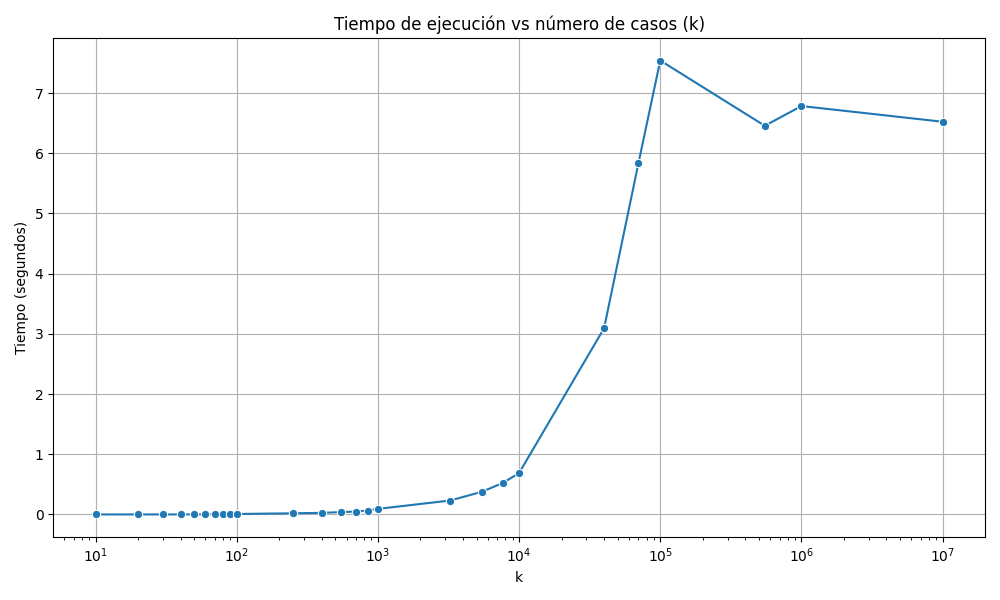
\includegraphics[width=0.8\textwidth]{../code/brute_force/data/plots/tiempo_vs_k.png}
    \caption{Tiempo de ejecución vs número de casos $k$ para algoritmo de fuerza bruta.}
    \label{fig:bf-tiempo}
\end{figure}

En la Figura~\ref{fig:bf-memoria}, que representa el uso de memoria del algoritmo de fuerza bruta, se observan valores anómalos extremadamente altos (del orden de $10^{19}$ MB), debido a que se fijo tambien el valor de la memoria con $k$ mayor a $1.000$. Sin embargo, en general, el consumo de memoria no escala significativamente con $k$, dado que cada subproblema es procesado de forma independiente y no se almacenan estructuras auxiliares significativas.

\begin{figure}[H]
    \centering
    \includegraphics[width=0.8\textwidth]{../code/brute_force/data/plots/memoria_vs_k.png}
    \caption{Uso de memoria vs número de casos $k$ para algoritmo de fuerza bruta.}
    \label{fig:bf-memoria}
\end{figure}

Por otro lado, la Figura~\ref{fig:dp-tiempo} muestra el tiempo de ejecución del algoritmo de programación dinámica. En este caso, el algoritmo muestra un crecimiento mucho más controlado del tiempo de ejecución, manteniéndose por debajo de los 8 segundos incluso para $k = 10^7$. Esto es consistente con la complejidad $O(nm)$ de este enfoque, que resulta mucho más eficiente al aumentar la cantidad de casos.

\begin{figure}[H]
    \centering
    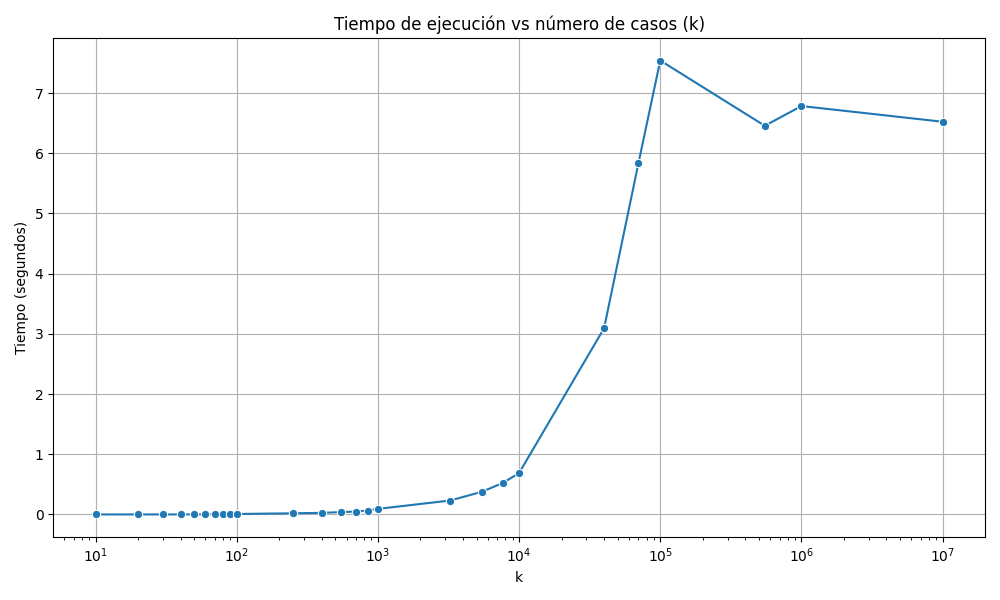
\includegraphics[width=0.8\textwidth]{../code/dynamic_programming/data/plots/tiempo_vs_k.png.png}
    \caption{Tiempo de ejecución vs número de casos $k$ para algoritmo de programación dinámica.}
    \label{fig:dp-tiempo}
\end{figure}

La Figura~\ref{fig:dp-memoria} muestra el uso de memoria del algoritmo de programación dinámica. Al igual que con el enfoque de fuerza bruta, se presentan algunos picos anómalos en los valores medidos. Estos valores no son consistentes con el comportamiento real del algoritmo, que debería tener un uso de memoria lineal respecto al número de casos y cuadrático respecto a la longitud máxima de las secuencias.

\begin{figure}[H]
    \centering
    \includegraphics[width=0.8\textwidth]{../code/dynamic_programming/data/plots/memoria_vs_k.png}
    \caption{Uso de memoria vs número de casos $k$ para algoritmo de programación dinámica.}
    \label{fig:dp-memoria}
\end{figure}

\newpage
\section{Conclusiones}
Los resultados obtenidos a lo largo del experimento permiten afirmar que el uso de programación dinámica representa una mejora significativa frente a la estrategia de fuerza bruta para resolver el problema de detección de diferencias entre dos secuencias. Esta mejora no solo se refleja en la reducción del tiempo de ejecución, sino también en la capacidad de escalar hacia entradas más grandes sin comprometer la viabilidad computacional del algoritmo.

El análisis comparativo entre ambos enfoques evidencia cómo la elección de una estrategia algorítmica adecuada puede determinar la eficiencia y aplicabilidad de una solución en contextos reales. La fuerza bruta, aunque conceptualmente clara, demuestra ser inviable para volúmenes altos de datos, mientras que la programación dinámica logra mantener un desempeño estable incluso en escenarios más exigentes.

De este modo, los resultados respaldan la necesidad de recurrir a enfoques más estructurados y optimizados para problemas combinatorios, especialmente cuando se espera escalar el uso del algoritmo. La información empírica recolectada no solo valida las complejidades teóricas discutidas, sino que también ilustra con claridad el impacto que tienen en la práctica.

Este trabajo, en definitiva, reafirma la importancia del análisis algorítmico desde una doble perspectiva: teórica y experimental, permitiendo una comprensión más integral del comportamiento de las soluciones frente a distintas condiciones de entrada.


\newpage

\newpage
\appendix


\section{Apéndice 1}
Aquí puede agregar tablas, figuras u otro material que no se incluyó en el cuerpo principal del documento, ya que no constituyen elementos centrales de la tarea. Si desea agregar material adicional que apoye o complemente el análisis realizado, puede hacerlo en esta sección.

\begin{mdframed} 
    Esta sección es solo para material adicional. El contenido aquí no será evaluado directamente, pero puede ser útil si incluye material que será referenciado en el cuerpo del documento. Por lo tanto, asegúrese de que cualquier elemento incluido esté correctamente referenciado y justificado en el informe principal.
 \end{mdframed}


 
\printbibliography

\end{document}


